%-- coding: UTF-8 --
\documentclass[UTF8]{ctexart}
\usepackage[utf8]{inputenc}
\usepackage{graphicx}
\usepackage{booktabs}
\usepackage{geometry}
\usepackage{fancyhdr}
\pagestyle{plain} % 此处为fancy时有页眉
\geometry{a4paper,scale=0.8}
\title{比亚迪公司估值分析与五种投资学模型联系与差异简析}
\author{楼家澍 2019191138}
\date{}
\begin{document}

\maketitle

\section{选择一个在深交所主板上市并且有过股票分红记录的公司}
\subsection{基本概况}
比亚迪是一家中国汽车品牌,创立于1995年,主要生产商务轿车和家用轿车和电池。由20多人的规模起步,2003年成长为全球第二大充电电池生产商,同年组建比亚迪汽车,比亚迪汽车遵循自主研发、自主生产、自主品牌的发展路线,矢志打造真正物美价廉的国民用车,产品的设计既汲取国际潮流的先进理念,又符合中国文化的审美观念。\par
比亚迪(002594)于2011年6月30日在深交所上市,属于汽车整车板块。是国内新能源汽车 领导企业(2018 年新能源汽车销售 24.78 万辆,数量略超特斯拉成全球第一), 目前比亚迪有四大主业,包括:汽车业务、电池业务、电子业务和云轨业务。 汽车业务是最主要的利润贡献来源(汽车业务收入占比 53\%)。截止2021年6月15日收盘,比亚迪股票价格为232.6元,相较其发行价18元已涨逾13倍。比亚迪上市以来,共分红七次,分红记录如下表所示:
\begin{center}
\begin{table}[h]
\centering
\begin{tabular}{@{}lllll@{}}
\toprule
分红日期       & 每股分红  &  &  &  \\ \midrule
2014-03-20 & 0.05  &  &  &  \\
2016-08-29 & 0.367 &  &  &  \\
2017-03-29 & 0.178 &  &  &  \\
2018-03-28 & 0.141 &  &  &  \\
2019-03-28 & 0.204 &  &  &  \\
2020-04-22 & 0.197  &  &  &  \\
2021-03-30 & 0.148 &  &  &  \\ \bottomrule
\end{tabular}
\end{table}
\end{center}\par
\subsection{股权结构}
实控人王传福,巴菲特持股逾十年。截至 2018 年三季报,比亚迪前十大股东持股 78.56\%,其中实际控制人王传福 (公司董事长)持股 18.79\%,公司副董事长吕向阳持股 8.77\%,伯克希尔·哈 撒韦(巴菲特)持股 8.25\%(2008 年持股至今),公司董事夏佐全持股 3.89\%, 其余主要为机构持股。\par
\subsection{分析意义}
在中美贸易战日趋激烈的当今,在汽车行业,比亚迪拥有当之无愧的核心科技,其发展与生死存亡对于整个国家而言尤为重要。故接下来将针对比亚迪股票的估值进行分析。
\section{使用单指数模型,计算该公司的 Beta 值}
$\beta$系数也称为贝塔系数(Beta coefficient),是一种风险指数,用来衡量个别股票或股票基金相对于整个股市的价格波动情况。要计算beta值,我们需要先选取一个指数作为参考,由于比亚迪在深圳交易所上市,故我们选取自2011年6月30日起的深证指数作为参考,如下图:\par
\begin{center}
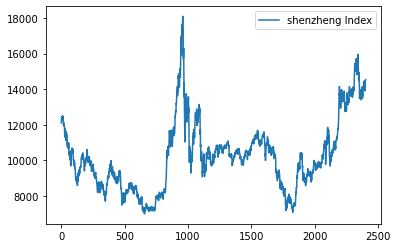
\includegraphics[scale=0.6]{下载 (10).png}
\end{center}\par
基于:\par
$$r_{it} = \alpha_{i} + \beta_{i}r_{mt}$$\par
我们以$r_{it}$为因变量,$r_{mt}$为因变量,对数据进行回归。结果如下:
\begin{center}
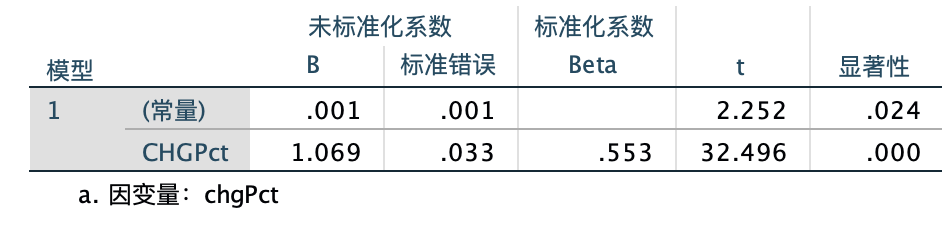
\includegraphics[scale=0.6]{截屏2021-06-16 下午9.38.52.png}
\end{center}\par
即$\beta$=1.069,由于$P-Value<0.000$,故该回归结果显著,具有统计学意义。
为了进一步验证回归结果,我们采用方差-协方差法再次计算$\beta$。\par
排除量纲对计算结果的影响,我们采用深证指数与比亚迪每日15:00收盘相比上一日价格变动作为参数。分别计算深证指数的方差以及深证指数和比亚迪的协方差。计算过程与结果如下:
\begin{center}
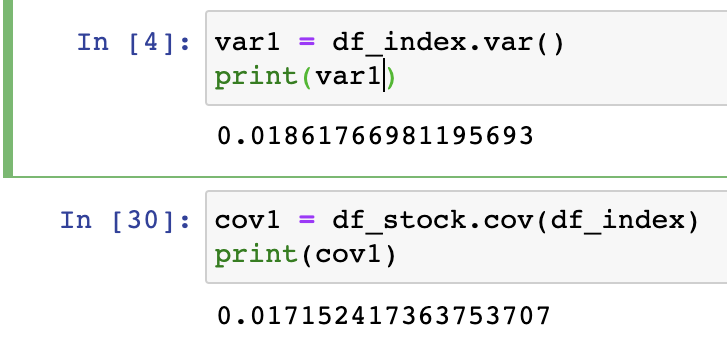
\includegraphics[scale=0.6]{截屏2021-06-16 下午9.46.35.png}
\end{center}\par
随后利用:\par
$$\beta = \frac{\sigma ^{2}}{cov}$$\par
计算得到比亚迪在深证指数中的$\beta$值为0.922,与上述回归结果相差不大,进一步验证了二者的准确性。最终,我们取两者的平均值作为最后的$\beta$值,$\beta=0.9955$。
\section{解释你所计算出的 Beta 值跟国泰安数据库给出的 Beta 值为何不同}
通过查阅国泰安数据库,我们得到比亚迪公司年度beta值的数据\cite{ref5}:\par
\begin{center}
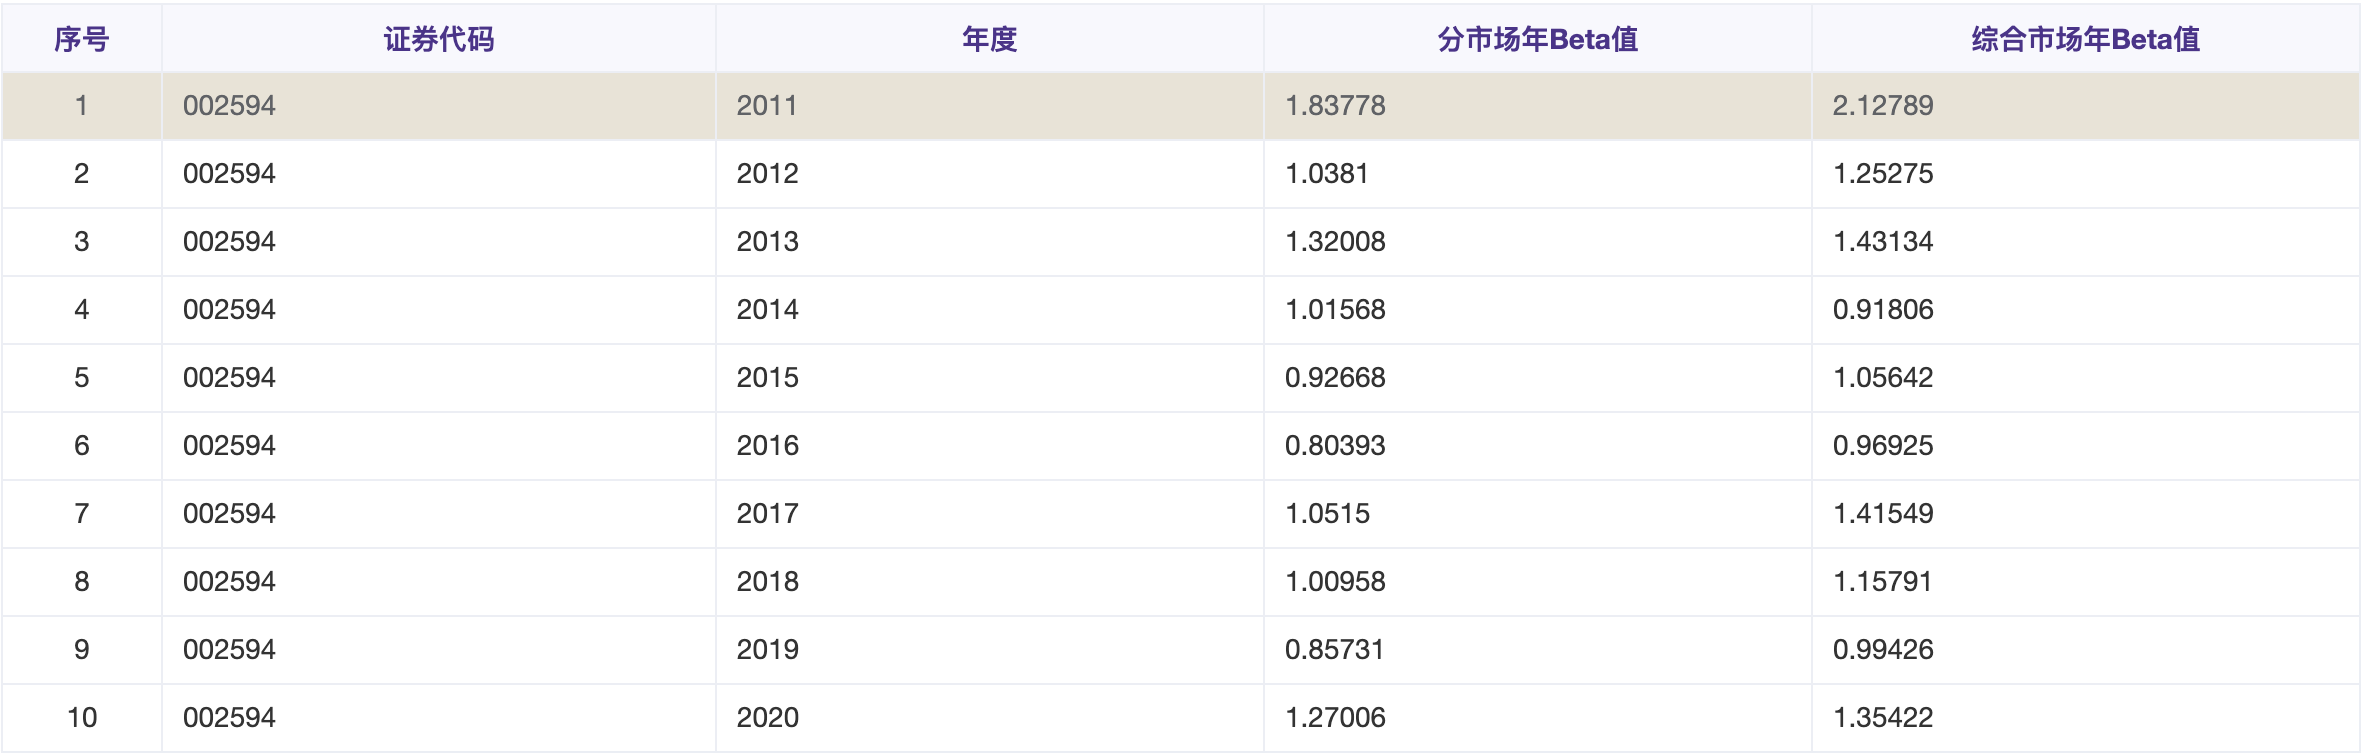
\includegraphics[scale=0.3]{截屏2021-06-16 下午4.11.37.png}
\end{center}\par
与我们所计算出来的beta值要偏大一点。通过查阅国泰安数据库的字段说明,我们发现,我们所计算beta的方法是不相同的。国泰安数据库采用单指数模型\cite{ref4}:\par
$$r_{it} = \alpha_{i} + \beta_{i}r_{mt} + \varepsilon _{it}$$\par
其中:$r_{it}$为第$i$只股票的收益率,$r_{mt}$为$t$时刻的市场回报率\par
$$\hat{\beta} = \frac{\sum_{t=1}^{T} (r_{it}-\bar{r}_{it})(r_{mt}-\bar{r}_{mt})}{\sum_{t=1}^{T}(r_{mt}-\bar{r}_{mt})^{2} } $$\par
国泰安数据库利用回报率进行回归分析,采用线性拟合从而得到beta值。该方法考虑了公司不确定因素,拥有更强的解释性。而上题计算得到的beta值仅仅是从统计学意义上考虑两者的偏差程度。故两者存在误差\cite{ref1,ref2}。\par
\section{基于第二部分的 Beta,使用 CAPM 模型为所选公司确定一个合适的回报 
率}
根据CAPM模型,单个股票的预期回报率公式如下:
$$\bar{r}_{a} = r_{f}+\beta_{a}(\bar{r}_{m}-\bar{r}_{f})$$
其中$\bar{r}_{a}$表示股票的预期回报率,$r_{f}$表示无风险回报率,$\beta_{a}$代表该股票的beta值,$\bar{r}_{m}$代表市场的平均回报率。\par
本文选取三个月存款利率作为无风险利率。由于我国目前尚无统一的无风险利率标准,许多学者选择存款利率作为无风险利率\cite{ref3}。\par
查阅资料得,中国银行三个月整存整取利率为1.350$\%$,故我们取$r_{f}=$1.350$\%$。由于指数会根据市值大小进行加权编制,故很难真实反映实际市场收益率。而被动型指数基金则不追求超越市场收益,只追求获取平均收益。故被动型指数基金的涨幅在一定程度上可以反映市场的平均收益率。我们选取易方达深证100ETF(159901),其近三年的总收益为69.13$\%$,平均收益为23$\%$.故我们令$\bar{r}_{m}$ = 23$\%$\par
由上述数据,我们求得比亚迪的预期回报率:\par

$\bar{r}_{a} =1.350$\%$ + 0.9955*(23$\%$ - 1.350$\%$) = 22.90\%$
而比亚迪在10年间股票涨幅逾13多倍,从该角度看比亚迪被高估了。

\section{预测所选公司股息的增长率}
我们从比亚迪公司的历史数据开始分析,得到比亚迪公司股息增长如下:
\begin{center}
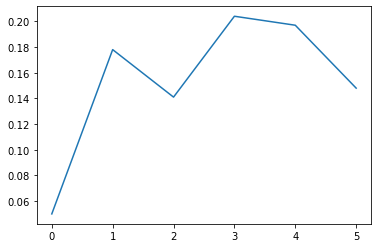
\includegraphics[scale=0.6]{下载 (16).png}
\end{center}\par
发现股息大致呈波动上升趋势。由于股息是公司业绩与发展的真实反映,我们再取以下公司财务数据以及宏观经济数据进行分析:
\begin{center}
\begin{table}[h]
\centering
\begin{tabular}{@{}lllllll@{}}
\toprule
日期        & 业绩    & PE     & beta & GDP   & 深证指数涨幅 & 分红    \\ \midrule
2014/3/20 & 4.34  & 56.48  & 0.99 & 64.4  & 33.8   & 0.05  \\
2016/8/29 & 50.52 & 27.74  & 1.01 & 74.36 & 14.72  & 0.367 \\
2017/3/29 & 40.66 & 47.68  & 0.98 & 83.2  & -3.54  & 0.178 \\
2018/3/28 & 27.8  & 68.34  & 1    & 91.93 & -33.25 & 0.141 \\
2019/3/28 & 16.14 & 80.55  & 0.99 & 98.65 & 35.89  & 0.204 \\
2020/4/22 & 42.34 & 125.19 & 1.03 & 101.6 & 35.3   & 0.06  \\
2021/3/30 &       &        & 1.06 &       &        & 0.148 \\ \bottomrule
\end{tabular}
\end{table}
\end{center}\par
随后我们借助SPSS对数据进行多元线性回归\cite{ref6},得到的结果如下:
\begin{center}
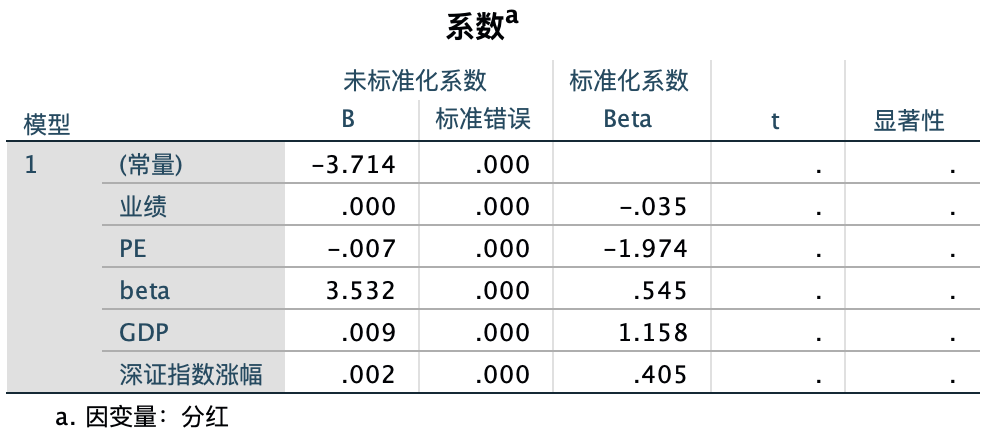
\includegraphics[scale=0.5]{截屏2021-06-17 上午11.48.29.png}
\end{center}\par
即:分红 = 0.35业绩-1.974PE+0.545$\beta$+1.158GDP+0.405深证指数涨幅\par
由同花顺数据,比亚迪公司2022年预测利润将增长35\%,假设其他数据不变,利用上述公式我们可以得到,2020年的分红预测值约为0.1823,相比2021年增长23.18\%
\section{ 给定股息年增长率为 1.2\%,利用股利贴现模型预测所选公司的股票价格}
根据稳定增长的股利模型:
$$V_{0} = \frac{D_{1}}{(r-g)}$$\par
根据第四题的结果,取r = 22.90\%。取2020年为$t_{0}$时刻,又因为已知$g = 1.2\%$我们将数据代入公式,得到:
$$V_{0} = \frac{0.148}{(3.13\%-1.2\%)} = 7.67$$\par
即如果你是为了通过股息获取收益,则比亚迪股票2020年的理论价格应该是7.67元每股\par
这个价格相较于比亚迪200多元的现价,显然低了太多了。由文献得知\cite{ref7}。股利贴现模型对我国股票价格几乎没有解释力,这与成熟资本市场有较大差异。说明我国资本市场的效率有待提高。由于成熟资本市场已有数百年的发展历程,因此成熟资本市场的研究中都假定其资本市场有效, 亦即它们用股票的价格来代表股票的内在价值,通过分析股票价格与不同模型预测价值的相关性而判定不同股权估价模型的有用性。而我国股票市场发展仅有20余年历史,暂时还不具备很强的有效性。
\section{请对你所选公司的股票提供投资建议}
\subsection{短期}
受华为造车概念,特斯拉概念等热点炒作影响。比亚迪的股票最近出现暴涨。而近日,涨幅有所放缓。通过查阅资料,比亚迪股票今日持仓平均成本为219元,股价在成本附近波动,抛压较强,向上突破阻力大。另外,港股比亚迪近日跌幅严重,出现了港股与A股背离的现象。以上指标提示近期以止盈止损为主,不建议买入股票。
\subsection{中期}
由于股价上涨放缓,且近日走出双头走势,属于一种头部盘整形态。预计中期见顶,暂时没有建仓时机,在中期股价很难创出新高。已经持有该股票的投资者可以继续坚定持有,而预计投资期限在1~2年的投资者暂时不要买入该股票。
\subsection{长期}
比亚迪是国内新能源汽车龙头。2018 年在国内车市整体表现不加的情况下,比 亚迪汽车逆势上扬,全年累计销售52.07万辆,同比增长 27.09\%,首度突破 50 万辆。其中新能源汽车销量为 24.78 万辆,同比 2017 年销量大幅增长 118\%, 为比亚迪 18 年销量逆势上扬带来强大增长动力。比亚迪连续 5 年成为国内新能 源汽车销量第一,且连续 4 年成为全球新能源汽车销量冠军。根据公司公告, 比亚迪新能源乘用车2018年销量 22.72 万辆,市场占有率达 22.63\%。凭借新 一代“龙脸”设计和科技加持,比亚迪有望迎来传统+新能源车两翼联动发展。\par
由于比亚迪公司成立时间不长,分红相较于同价股票比较不慷慨。但随着公司的发展与利润的提高,我们预计比亚迪公司的分红能够以20~30\%的比例增长。从长远角度看,汽车行业是国民行业,拥有自己的民族汽车企业是国家的立国之本。故我们建议在任何时点买入比亚迪,并长期持有,从公司发展与国家经济发展的双重红利获得价值收益。\par
\section{ 解释单因素模型、多因素模型、CAPM 模型、APT 模型和 Famma-
 French 模型的联系和差异}
 \subsection{单因素模型与多因素模型}
\subsubsection{单因素模型}
单因素模型认为,资产收益的不确定性有两个来源:宏观经济因素和公司特有因素。其中,可能的宏观经济因素包括国内生产总值增长和利率等。由此得到资产收益的公式为:\par
$$r_{it} = \alpha_{i} + \beta_{i}r_{mt} + \varepsilon _{it}$$\par
单因素模型的优势:\par
a.相对于马科维茨模型,简化协方差矩阵的估计;\par
b. 相对于马科维茨模型,强化风险溢价的估计;\par
c.为宏观分析和证券分析提供了分析框架。\par
单因素模型的缺点:\par
a.把模型定性为线性关系,但实际情况是否如此,还有待检验和确认。有可能实际情况并非线性关系。\par
b.把各种复杂的宏观经济因素只抽象成一个因素,并不符合实际运行情况,实际的市场中宏观经济因素应该包括各种因素,需具体去分析。\par
\subsubsection{多因素模型}
多因素模型则是在单因素模型的基础上,将宏观因素分解为多个因素进行阐述,因为使用包含多个因素的多因素模型来解释证券收益更加合理。其中的宏观因素有多个,例如:国内生产总值、预期通货膨胀、利率。并且,可以使用多元回归来估计每个因素的贝塔值或因子载荷。由此得到资产收益的公式为:
 $$r_{it} = \alpha_{i} + \beta_{iGDP}r_{mt} + \varepsilon _{it}$$\par
即在单因素模型的基础上引入了更多因素,使得其更贴近真实情况。\par
多因素模型的优势:\par
a.相对于单因素模型和CAPM模型,多因素模型提供了一种更加丰富的方法去处理风险补偿问题。\par
b.多因素模型可以更具体、精确地捕捉不同宏观经济因素的变化对特定证券收益的影响。\par
多因素模型的缺点:\par
a.与单因素模型一样,把模型定性为线性关系,但实际情况是否如此,还有待检验和确认。\par
b.把宏观经济因素分解为若干个具体因素后,其测算与估计的精确度是较难把握的。\par
\subsubsection{联系与差异}
单因素模型和多因素模型都认为证券的收益来源于其风险,但是多因素模型认为这个风险不仅仅来源于证券本身,同时也来自于其他很多的外部因素。例如投资人的经济状况、市场情况等等。\par
总体上而言多因素模型是单因素模型的细化与改进,用更多的因素去逼近现实。
\subsection{CAPM模型与APT模型}
\subsubsection{CAPM模型}
资本资产定价模型(CAPM模型)假设所有投资者都按马克维茨的资产选择理论进行投资,对期望收益、方差和协方差等的估计完全相同,投资人可以自由借贷。基于这样的假设,资本资产定价模型研究的重点在于探求风险资产收益与风险的数量关系,即为了补偿某一特定程度的风险,投资者应该获得多少的报酬率。基于上述介绍,CAPM模型的表达式如下:\par
$$\bar{r}_{a} = r_{f}+\beta_{a}(\bar{r}_{m}-\bar{r}_{f})$$
\subsubsection{APT模型}
APT(Arbitrage pricing theory),即套利定价模型,是一种资产价格的估值模型,是资本资产定价模型(CAPM)的替代理论。其理论基础是一项资产的价格是由不同因素驱动,将这些因素乘上该因素对资产价格影响的贝塔系数,加总后,再加上无风险收益率,就可以得出该项资产的价值。
\subsubsection{联系与差异}
与资本资产定价模型一样,套利定价理论假设:

  1.投资者有相同的投资理念;

  2.投资者是回避风险的,并且要效用最大化;

  3.市场是完全的。

  与资本资产定价模型不同的是,套利定价理论不包括以下假设:

  1.单一投资期;

  2.不存在税收;

  3.投资者能以无风险利率自由借贷;

  4.投资者以收益率的均值和方差为基础选择投资组合。\par
资本资产定价模型(CAPM)和套利定价理论(APT)是关于资本市场均衡的两个比较著名的模型。二种模型虽然在解释的角度、基本假设、方法、以及适用范围上均有重大区别,但是殊途同归,它们得出的结论是一致的:期望收益与风险之间存在着正相关的关系。\par
\subsection{Famma-
French 模型}
\subsubsection{Famma-
French 模型简介}
Fama和French 1993年指出可以建立一个三因子模型来解释股票回报率。模型认为,一个投资组合(包括单个股票)的超额回报率可由它对三个因子的暴露来解释,这三个因子是:市场资产组合(Rm−Rf)、市值因子(SMB)、账面市值比因子(HML)。这个多因子均衡定价模型可以表示为:
$$E(R_{it})-R_{ft}=\beta_{i}[E(R_{mt}-R_{ft}]+siE(SMB_{t})+hiE(HMI_{t})$$\par
其中$R_{ft}$表示时间$t$的无风险收益率;$R_{mt}$表示时间$t$的市场收益率;$R_{it}$表示资产$i$在时间$t$的收益率;$E(R_{mt}) − Rft$是市场风险溢价,$SMB_{t}$为时间$t$的市值因子的模拟组合收益率,$HMI_{t}$为时间$t$的账面市值比因子的模拟组合收益率。\par
\subsubsection{联系与差异}
与上述四个模型不同的是,上述四个模型认为,股票的期望收益只与市场的系统风险有关。但是,Famma-
French 模型认为,股票的收益还与其市场价值有关。\par
除此之外,Famma-
French 模型还放弃了绝对理性市场的假设,他认为市场是有限理性的。即用“社会人”来代替“经济人”,使得模型更贴近现实社会。\par
\subsection{结论}
以上五个模型从简单到复杂,从一般到特殊,从理想到现实,一步一步地变得更为精确。而始终坚持不变的是他们都认为证券的收益性来源于它的风险性,而逐步完善起来的是风险的种类与细节。\par
我们可以发现的是,越现代的投资学模型越能体现出人性的缺陷与不完善性\cite{ref8}。而我们却不能去指责人性的残缺,应该转而去思考我们所谓的理想市场是不是从一开始就是错的。毕竟这一个个不完善的所谓“社会人”才是构成我们市场的原子,你不能用一个完美的假说去否定现实的存在。所以在投资学领域,对人性的逐步深入研究必然是一个永恒的话题。\par

\begin{thebibliography}{99}
\bibitem{ref1} 孙凯.国内证券市场Alpha套利策略实证研究[D].对外经济贸易大学,2014.
\bibitem{ref2} 刘永阔.基于CAPM模型的资产定价问题求解以及模型改进[J].商讯,2021(07):174-175.
\bibitem{ref3} 金梦影.资本资产定价(CAPM)模型在中国证券市场的适用性研究[J].中国乡镇企业会计,2020(06):9-10.
\bibitem{ref4} 国泰安数据库.风险评价系数β 数据库说明书
\bibitem{ref5} 国泰安数据库.风险评价系数β
\bibitem{ref6}孙佳宁.基于多元回归模型研究沪深300股指与CPI之间的影响关系[J].大众投资指南,2021(10):16-17.
\bibitem{ref7}张景奇,孟卫东,陆静.股利贴现模型、自由现金流量贴现模型及剩余收益模型对股票价格与价值不同解释力的比较分析——来自中国证券市场的实证数据[J].经济评论,2006(06):92-98.
\bibitem{ref8}高增亮,张俊瑞.行为金融视角下投资者情绪对财务重述行为的影响[J].中南财经政法大学学报,2019(03):85-93+159.
\end{thebibliography}
\end{document}
